\begin{center}
    \textbf{Geração 1}
\end{center}

\begin{figure}[h]
    \centering
    \label{fig:geracao01}
    
    \begin{tabular}{rl}
        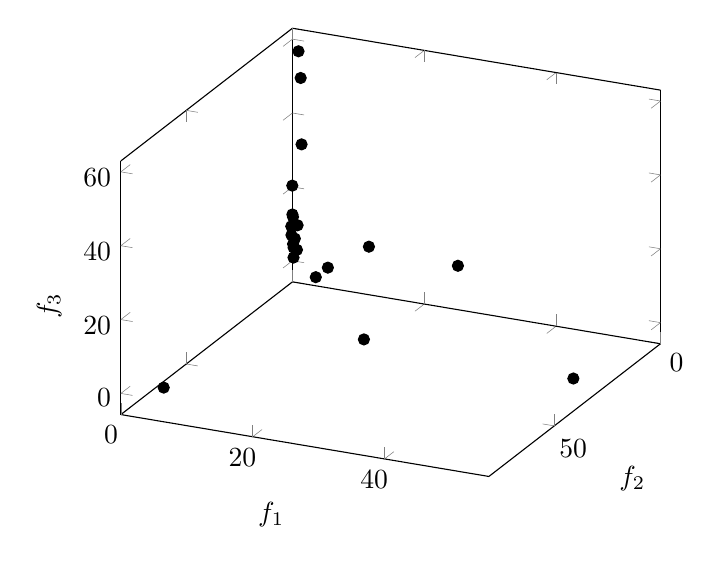
\begin{tikzpicture}[scale=1.0]
        	\begin{axis}[xlabel=$f_2$, ylabel=$f_1$, zlabel=$f_3$, view/h=115]
        		
    			\addplot3[style={dashed}]coordinates {
    			    (0., 0., 0.5) (0., 0.5, 0.) (0.5, 0., 0.) (0., 0., 0.5)
    			};
    			
    			\addplot3[style={dashed}]coordinates {(0., 0.1, 0.4) (0.4, 0.1, 0.)};
    			\addplot3[style={dashed}]coordinates {(0., 0.2, 0.3) (0.3, 0.2, 0.)};
    			\addplot3[style={dashed}]coordinates {(0., 0.3, 0.2) (0.2, 0.3, 0.)};
    			\addplot3[style={dashed}]coordinates {(0., 0.4, 0.1) (0.1, 0.4, 0.)};
    			
    			\addplot3[style={dashed}]coordinates {(0.4, 0., 0.1) (0.4, 0.1, 0.)};
    			\addplot3[style={dashed}]coordinates {(0.3, 0., 0.2) (0.3, 0.2, 0.)};
    			\addplot3[style={dashed}]coordinates {(0.2, 0., 0.3) (0.2, 0.3, 0.)};
    			\addplot3[style={dashed}]coordinates {(0.1, 0., 0.4) (0.1, 0.4, 0.)};
    			
    			\addplot3[only marks] coordinates {
            		(0.132104, 0.125725, 11.950734) (0.326311, 0.197952, 4.729548) (0.404188, 0.121029, 12.739288) (1.741078, 5.933249, 0.683002) (0.236987, 0.237160, 1.030411) (6.894477, 5.762771, 0.342752) (2.317222, 0.923250, 4.863639) (1.425533, 0.309608, 7.677182) (0.864683, 0.959345, 3.618312) (1.109343, 0.332909, 20.929687) (0.451953, 1.063746, 57.231064) (80.785634, 6.500717, 3.529559) (35.688217, 22.341444, 1.274403) (1.896716, 0.433023, 10.283637) (1.066062, 1.728381, 32.500493) (1.646791, 1.310902, 10.725314) (3.595265, 1.520277, 8.043359) (41.017074, 55.836087, 3.110179) (4.582401, 26.581514, 8.646189) (9.536530, 14.673468, 12.447320) (1.880235, 1.853029, 50.874195) 

        		};
        	\end{axis}
	    \end{tikzpicture}
	    &
	    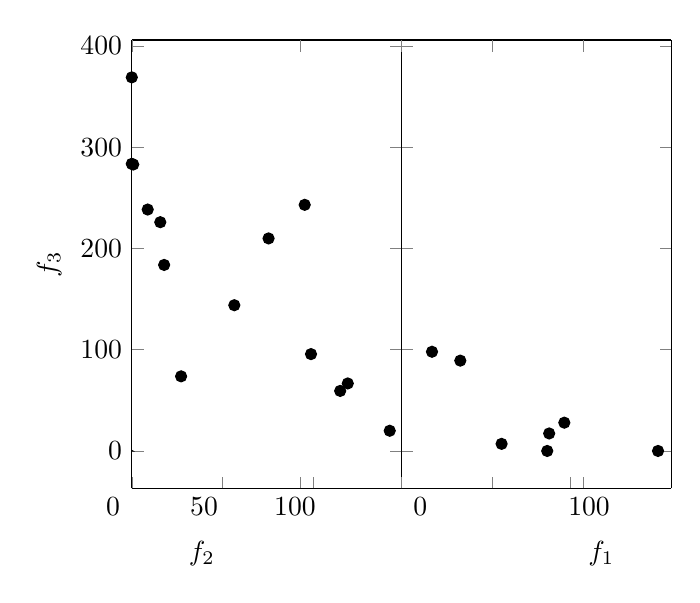
\begin{tikzpicture}[scale=1.0]
        	\begin{axis}[xlabel=$f_2$, ylabel=$f_1$, zlabel=$f_3$, view={45}{0}]
        		
    			\addplot3[style={dashed}]coordinates {
    			    (0., 0., 0.5) (0., 0.5, 0.) (0.5, 0., 0.) (0., 0., 0.5)
    			};
    			
    			\addplot3[only marks] coordinates {
            		(0.201382,0.639630,282.807806)(3.725762,5.416148,238.355405)(21.377820,83.168506,95.622558)(4.833895,55.546046,143.890665)(23.630069,3.760357,73.665477)(148.372971,59.253174,7.018980)(112.671235,6.571695,66.655111)(144.707050,91.395954,17.275659)(99.854101,15.887599,59.285671)(138.562523,96.858265,0.000000)(0.000000,0.000000,283.462850)(1.734380,100.592399,243.006254)(14.787484,3.237811,183.660386)(92.800833,52.845645,19.950849)(14.824096,0.920929,225.857233)(141.011831,159.877050,0.000000)(0.000000,0.000000,368.853860)(121.181027,125.718632,27.922188)(71.606499,3.888244,209.836325)(34.032717,157.989311,89.175723)(100.476088,69.623546,97.935049)


        		};
        	\end{axis}
	    \end{tikzpicture}
	\end{tabular}
    
\end{figure}

